\documentclass[../main.tex]{subfiles}

\graphicspath{{\subfix{../figures/}}}

\begin{document}

\Gls{cryoem} is a novel imaging technique that involves \glspl{tem} to analyze frozen samples. Differing from conventional optical microscopes, \glspl{tem} employ an electron beam instead of light, enabling them to capture of images at significantly higher resolutions. Consequently, \gls{cryoem} has gained popularity for analyzing biological molecules such as proteins and viruses\cite{chemistry_world_cryoem}. In this regard, \gls{spa} constitutes a set image acquisition and processing techniques that facilitates such a task. In this process, a significant amount of two-dimensional images are utilized to elucidate the three-dimensional structure of the specimen under study.

However, \glspl{tem} subject the sample to very extreme conditions, such as near perfect vacuum and high-energy electrons. Thus, the sample is frozen before entering the microscope. This helps to maintain it intact when exposed to such environment. The sample freezing is performed in a matter of milliseconds, in a process known as plunge-freezing. This process avoids the formation of ice crystals, which would diffract the electron beam. This technique was awarded with the 2017 Nobel Prize in Chemistry\cite{chemistry_world_cryoem}\cite{nobel2017}.

%\begin{figure}[htbp]
%    \centering
%    \begin{subfigure}[b]{0.3\textwidth}
%         \centering
%         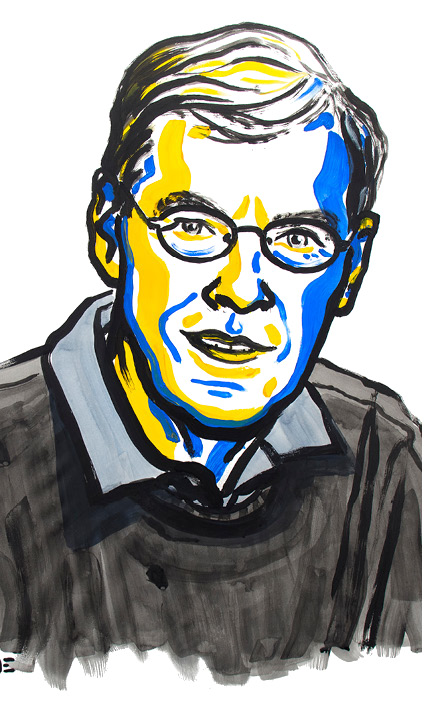
\includegraphics[width=\textwidth]{nobel2017/Richard Henderson}
%         \caption{Richard Henderson}
%         \label{fig:1:nobel2017:richard}
%    \end{subfigure}
%    \hfill
%    \begin{subfigure}[b]{0.3\textwidth}
%         \centering
%         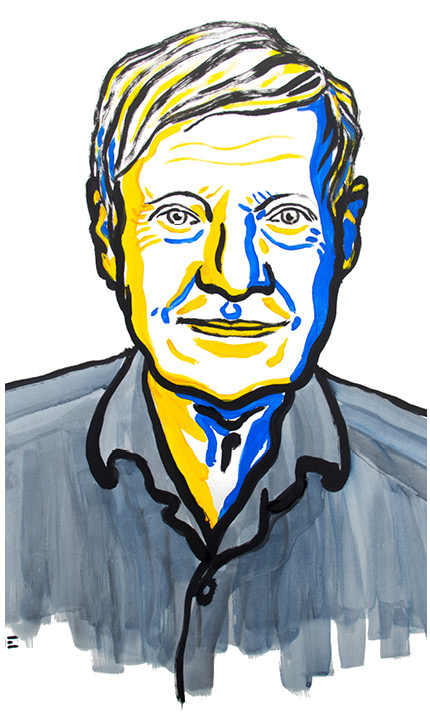
\includegraphics[width=\textwidth]{nobel2017/Joachim Frank}
%         \caption{Joachim Frank}
%         \label{fig:1:nobel2017:joachim}
%    \end{subfigure}
%    \hfill
%    \begin{subfigure}[b]{0.3\textwidth}
%         \centering
%         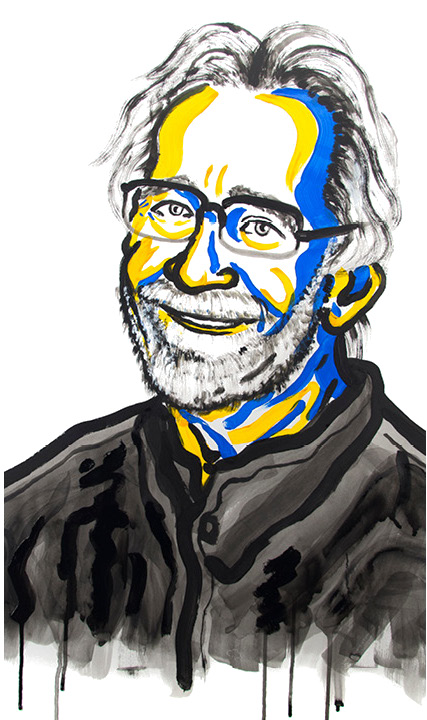
\includegraphics[width=\textwidth]{nobel2017/Jacques Dubochet}
%         \caption{Jacques Dubochet}
%         \label{fig:1:nobel2017:jaques}
%    \end{subfigure}\\
%    Images obtained from: \cite{science_nobel}
%    \caption{2017 Nobel Prize in Chemistry}
%    \label{fig:1:nobel2017}
%\end{figure}

In \gls{spa}, thousands of samples are spread on a copper or gold grid, each of them holding a random orientation. Individually referred to as ``particles'', a extensive amount of 2D projections can be used to mathematically infer the 3D structure of the specimen\cite{cryoem101}. This process is hindered by many artifacts such as the poor \gls{snr} present in \gls{cryoem} images, which is in the order of $1/100$, this is, noise is much more prominent than the actual signal.

\begin{figure}[hbp]
    \centering
    \begin{subfigure}[b]{0.45\textwidth}
         \centering
         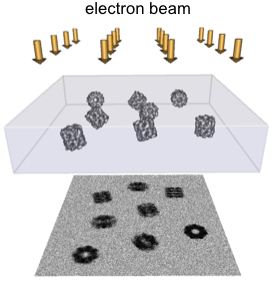
\includegraphics[width=\textwidth]{SPA/projection_reconstruction/acquisition}
         \caption{Image acquisition}
    \end{subfigure}
    \hfill
    \begin{subfigure}[b]{0.45\textwidth}
         \centering
         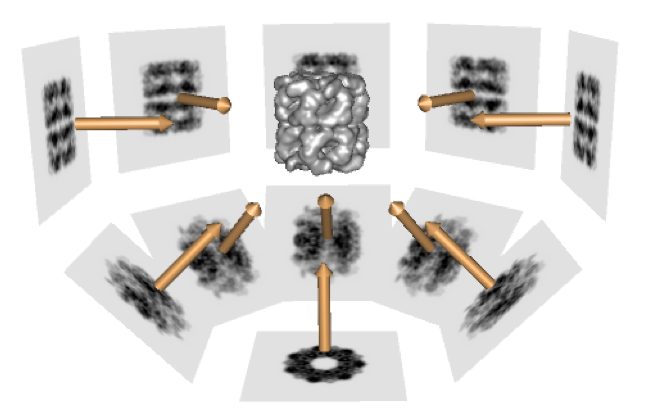
\includegraphics[width=\textwidth]{SPA/projection_reconstruction/reconstruction}
         \caption{Reconstruction}
    \end{subfigure}\\
    Images obtained from: \cite{greg}
    \caption{SPA image acquisition and structure reconstruction}
    \label{fig:1:acquisition_reconstruction}
\end{figure}

The mathematical models used for reconstruction assume that all projections originate from the same 3D structure. Nevertheless, this does not hold true in many real world cases. In instances where a dataset comprises diverse structures, known as heterogeneous, projections must be categorized based on their corresponding structures, which are unknown. This procedure, known as 3D classification, forms the central theme of this thesis.

This End of Masters Thesis is the author's second work on \gls{cryoem}. Previously, on July 2023, he presented a work on fast image alignment algorithms\cite{zarrabeitia2023}. Although this project shares the context (\gls{cryoem}) with the previous one, the actual problem is completely different. Nevertheless, some introductory sections were borrowed from the preceding publication.

This project was conducted within the \gls{bcu} research group, situated at the \gls{cnb} under the \gls{csic}. This research group is actively involved in the development of two software suites related to \gls{cryoem}, namely Xmipp and Scipion. Xmipp focuses on implementing image processing algorithms, while Scipion serves as a framework facilitating seamless interoperability among cutting-edge image processing suites. Consequently, the software developed in this project will be incorporated into Xmipp and integrated into Scipion.

\section{Heterogeneity in CryoEM and 3D classification}
\subfile{1.1-3D classification}

\section{Objectives}
\subfile{1.2-Objectives}

\section{Structure of the document}
\subfile{1.3-Structure}

\end{document}
 